\section*{\begin{tabular*}{\linewidth}{@{}l @{\extracolsep{\fill}} r@{}}
Nr.~2 & MLB~85/1-3-2\\
\end{tabular*} 
}

\textsf{\textbf{Maluba (Lua; Fpl.~230)}}

\vspace{1em}

\noindent\begin{tabular}{@{}rl@{}}
\textbf{Feldarbeit:} & \textbf{08.09.1985 (F. Nikulka)} \\ 
\textbf{Abb.:} & \textbf{\ref{fig:MLB85-1-3-2_NordProfil}--\ref{fig:Fragmenierung_MLB85-132}} \\
\textbf{Tab.:} & \textbf{\ref{tab:MLB85-1-3-2_Funde}--\ref{tab:MLB85_1-3-3_14C-Daten}}\\
\textbf{Taf.:} & \textbf{26.9--27.8} \\ 
\textbf{Lit.:} & \textbf{\textsc{Eggert}~1987b} \\ 
\end{tabular}

% NOTES: MLB 85/104 == MLB 85/1-3-2

\paragraph{Grabung und Befunde}\hspace{-.5em}|\hspace{.5em}%
Direkt nordwestlich der Grube MLB~85/1-3-1 (Kat.-Nr.~1) wurde eine weitere, teilweise frei erodierte Grube erfasst.\footnote{Die abgesammelten Funde erhielten die Bezeichnung MLB~85/104. Aus dem Survey-Inventar stammt ein fragmentiertes Gefäß der Batalimo-Maluba-Gruppe (Taf.~26.9).} Während der Ausgrabung von MLB~85/1-3-1 wurde der Befund angeschnitten und als Komplex MLB~85/1-3-2 untersucht (Abb.~\ref{fig:MLB85_1_Zeichnung}--\ref{fig:MLB85_1_PlanaT70}). Im Zuge der Ausgrabung konnte die stratigraphische Relation zwischen den beiden Gruben nicht erfasst werden.\footnote{Während der Ausgrabung der Sekundärbestattung MLB~85/1-4-3 (Kat.-Nr.~3) wurde beobachtet, dass diese in die Verfüllung der Grube MLB~85/1-3-2 eingreift, also stratigraphisch jünger ist (Abb.~\ref{fig:MLB85-143}).} Die wannenförmige, bis etwa 0,7\,m unter die heutige Oberfläche reichende Grube MLB~85/1-3-2 hat steilschräge bis schräge Wandungen, die fließend in eine konvexe Sohle übergehen (Abb.~\ref{fig:MLB85-1-3-2_NordProfil}). Die Befundgrenzen sind verwaschen bis fließend.\footnote{Im Vergleich zu den scharfen Befundgrenzen der Gruben MLB~85/2 und MLB~85/103 (Kat.-Nr.~4--5) zeigen die verwaschenen Grenzen das höhere Alter der beiden, Keramik des Batalimo-Maluba-Stils enthaltenen Gruben MLB~85/1-3-1 und MLB~85/1-3-2 (Kat.-Nr.~1--2).} Im Gelände wurden keine \textit{Verfüllschichten} beschrieben, die vorliegenden Fotos legen jedoch mindestens vier unterschiedliche Verfüllpakete mit konvexen bis welligen Schichtgrenzen nahe (Abb.~\ref{fig:MLB85-1-3-2_NordProfil}).\columnbreak

\begin{table*}[tb]
	\centering
	{\footnotesize \begin{sftabular}{@{}lrrrr@{}}
\toprule
   \textbf{Fundkategorie} &  \textbf{Anzahl} &    \textbf{\%} &  \textbf{Gewicht (kg)} &    \textbf{\%} \\
\midrule
 gebrannter Lehm &       2 &   1,8 &          0,40 &  11,9 \\
         Keramik &     108 &  97,3 &          2,72 &  81,0 \\
           Stein &       1 &   0,9 &          0,24 &   7,1 \\
\bottomrule
\end{sftabular}
}
	\caption{MLB~85/1-3-2: Anteil verschiedener Fundmaterialien.}
	\label{tab:MLB85-1-3-2_Funde}
\end{table*}

Im zweiten Abtrag wurde im nördlichen Bereich eine ausgeprägte Holzkohlekonzentration erfasst. Unterhalb des dritten Abtrages, ab einer Tiefe von etwa 0,4--0,5\,m unter der Oberfläche ging die dunkle, schwarze Kernverfüllung (Abb.~\ref{fig:MLB85-1-3-2_NordProfil}: Schicht~2) langsam in einen braun-gelben, inhomogenen Mischbereich aus sandigem Lehm und Sand über (Abb.~\ref{fig:MLB85-1-3-2_NordProfil}: Schicht~3). Bis zu einer Tiefe von etwa 0,6\,m unter der Oberfläche trat in diesem Mischbereich auch noch Keramik auf. Ab etwa 0,77\,m war die Sohle (Abb.~\ref{fig:MLB85-1-3-2_NordProfil}: Schicht~4) erreicht. Im Planum wurde nur noch der anstehende gelbe Lehm beobachtet. Die Schichten~1--4 entsprechen in etwa den Niveaus der künstlichen Abträge.

\vspace{.5em}\noindent Nach der vorliegenden Fotodokumentation lässt sich folgender stratigrafischer Befund ableiten:\footnote{Im Gelände wurden Plana und Profile nicht beschrieben und auch gezeichnet.}
\begin{itemize}[leftmargin=*, labelindent=0.5em, noitemsep, topsep=0pt]
	\item [(1)] Stark dunkelgrauer, homogener Bereich (rezenter Oberboden oder Verfüllungsbereich); wenige Funde.
	\item [(2)] Dunkelgraue bis schwarze, fleckige Schicht mit hohem Fundaufkommen, durchzogen von etwa 0,1--0,2 m dicken, tief dunklen/schwarzen Bändern; enthält viele ziegelrote Brocken.
	\item [(3)] Hellgraue, fleckige Schicht; Mischbereich aus sandigem Lehm und Sand; enthält Hüttenlehm und Holzkohle.
	\item [(4)] Leicht vergraute Grubensohle; im Profil sind keine/kaum Funde sichtbar.
	\item [(5)] Anstehender, gelber Lehm.
\end{itemize}

\paragraph{Keramik\vspace{.5em}}\mbox{}\\
\begin{tabular}{@{}lrl@{}}
Ausgesondert: & 459\,g & \\
Bearbeitet: & 2263\,g & (83\,\%) \\
Insgesamt: & 2722\,g & \\
\end{tabular} 

\begin{figure*}[p]
	\centering
	\begin{subfigure}[t]{\textwidth}
		\centering
		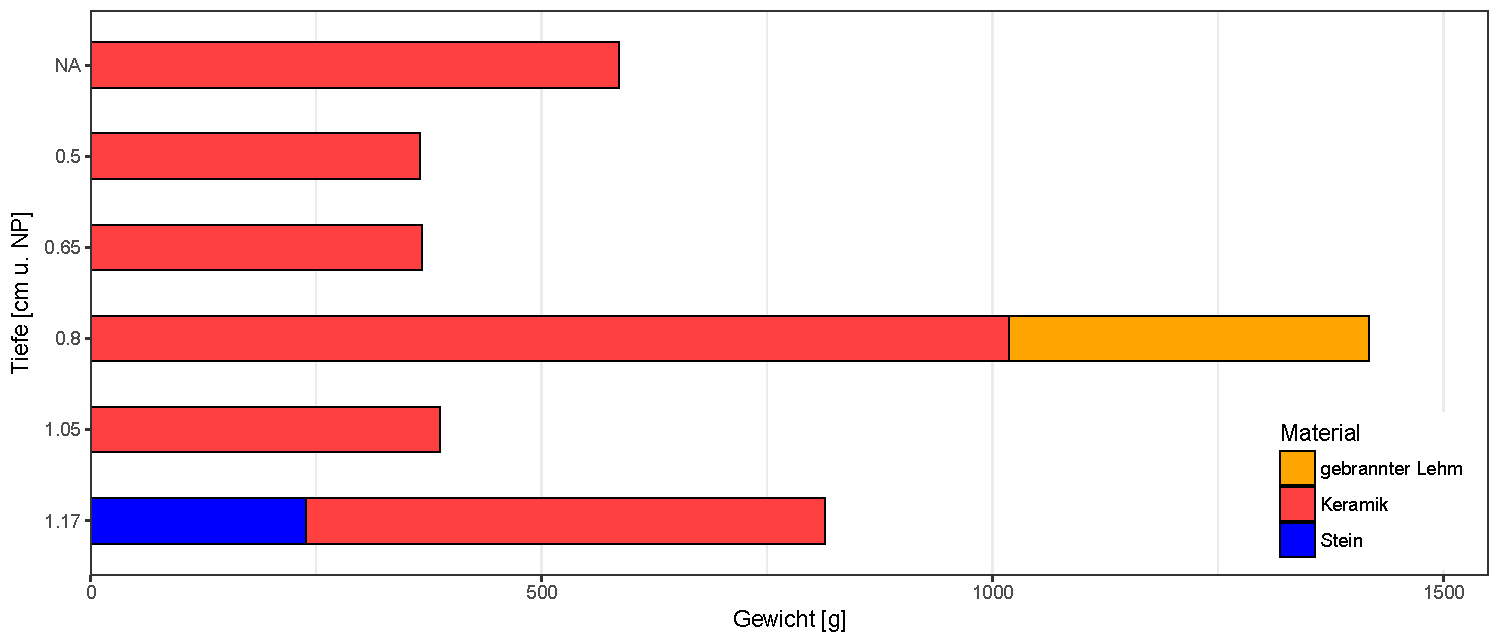
\includegraphics[width=\textwidth]{fig/9-2_MLB85-132_VerteilungFunde_R.pdf}
		\caption{Fundmaterial.\vspace{1em}}
		\label{fig:MLB85-132_VerteilungFunde}
	\end{subfigure}
	\begin{subfigure}[t]{\textwidth}
		\centering
		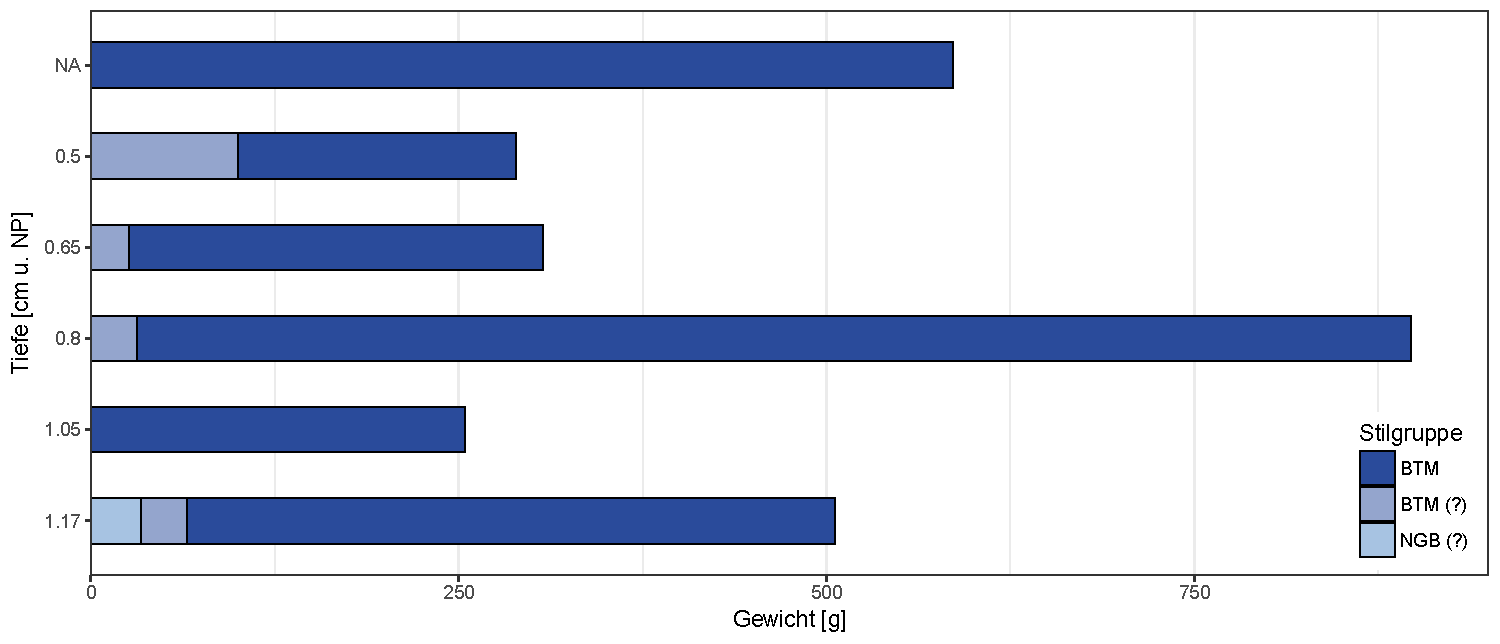
\includegraphics[width=\textwidth]{fig/9-2_MLB85-132_KeramikStilgruppen_R.pdf}
		\caption{Keramische Stilgruppen.\vspace{1em}}
		\label{fig:MLB85-132_KeramikStilgruppen}
	\end{subfigure}
	\begin{subfigure}[t]{\textwidth}
		\centering
		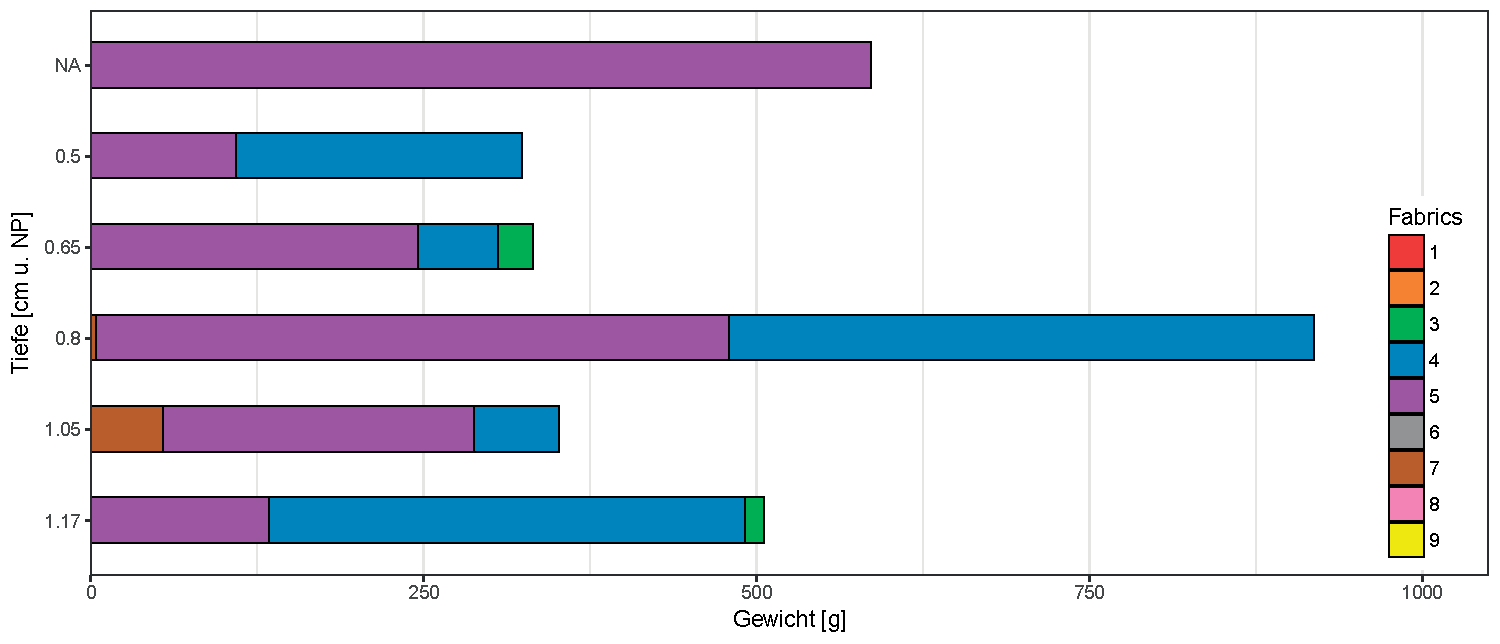
\includegraphics[width=\textwidth]{fig/9-2_MLB85-132_Fabrics_R.pdf}
		\caption{\textit{Fabrics}.}
		\label{fig:MLB85-132_VerteilungFabrics}
	\end{subfigure}
	\caption{MLB 85/1-3-2: Verteilung der Fundmaterialien (A), keramischen Stilgruppen (B) und \textit{Fabrics} (C) in den entsprechenden Tiefen der Grabung.}
	\label{fig:MLB85-132_Verteilung}
\end{figure*}

\vspace{1em}
\noindent Das keramische Inventar aus dem Befund MLB~85/1-3-2 kann bis auf ein Fragment komplett der Batalimo-Maluba-Gruppe (Kap.~\ref{sec:BTM-Gr}) zugerechnet werden. Es gibt nur sehr wenige, nicht näher ansprechbare Scherben, die eventuell jüngeren Gruppen angehören. Die Keramik bildet, zusammen mit jener aus der direkt benachbarten Grube MLB~85/1-3-1 (Kat.-Nr.~1), den Grundstock für den Formenkatalog des Batalimo-Maluba-Stils. Die einzeln aufgenommenen, diagnostischen GE repräsentieren mehr als 80\,\% des Inventars aus der Grube. Das Gros der Funde lag an der Sohle der dunklen, stark heterogenen Schicht~2, die bis etwa 0,44\,m unter die Oberfläche reichte und vor allem im dritten Abtrag erfasst wurde (Abb.~\ref{fig:MLB85-132_VerteilungFunde}). Die darunter liegende, hellere, durchmischte Schicht~3 beziehungsweise der vierte Abtrag erbrachte weniger Fundmaterial. An der Sohle der Grube steigt das Keramikaufkommen wieder leicht an.\footnote{Im West--Ost durch den Befund laufenden Profil (Abb.~\ref{fig:MLB85-132_W-O-Prof}) ist in dieser Schicht der Rand einer Schale des Typs E5 zu erkennen.}

\begin{figure*}[tb!]
	\centering
	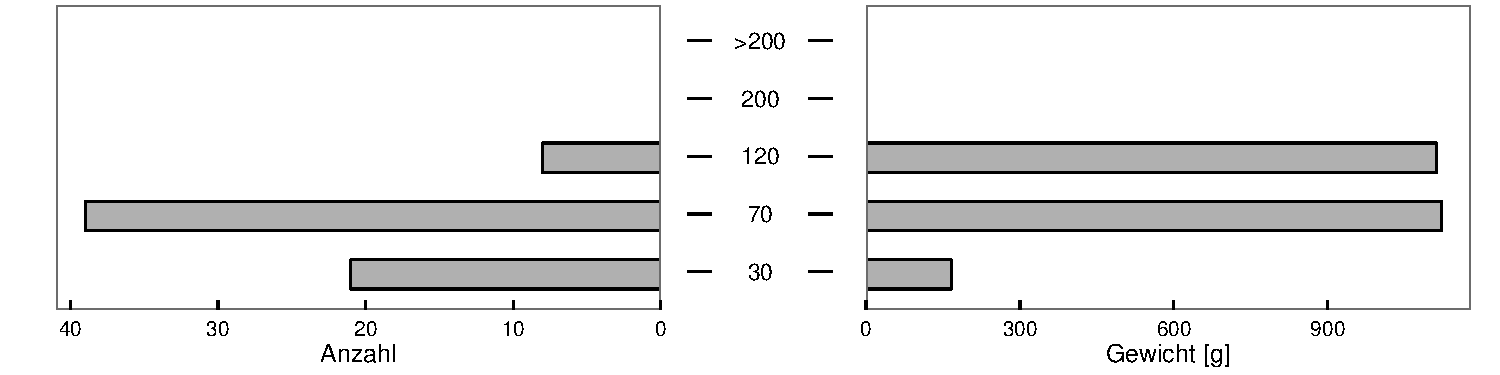
\includegraphics[width=\textwidth]{fig/9-2_MLB85-132_Fragmentierung_2.pdf}
	\caption{MLB~85/1-3-2: Fragmentierungsgrad der Scherben (n~=~68; Größenklassen siehe Anm.~\ref{ftn:Keramik_Fragmentierung}).}
	\label{fig:Fragmenierung_MLB85-132}
\end{figure*}

\begin{table*}[tb!]
	\vspace{1em}
	\centering
	{\footnotesize
		\begin{sftabular}{@{}p{.125\textwidth}p{.125\textwidth}p{.25\textwidth}p{.2\textwidth}p{.15\textwidth}@{}}
			\toprule 
			\textbf{Lab-Nr} & \textbf{Datum (bp)} & \textbf{Datum (2-Sigma)} & \textbf{Abtrag} & \textbf{Tiefe (unter NP)} \\ 
			\midrule 
			KI-2445 & 2140\( \pm \)200 & 764--680 v.~Chr. (3,6\,\%); 674 v.~Chr.--245 n.~Chr. (91,8\,\%) & 3 (MLB~85/1-3-2-3; HK 33) & 0,65--0,8\,m \\ 
			GrN-13585 & 1990\( \pm \)60 & 166 v.~Chr.--129 n.~Chr. & 4 (MLB~85/1-3-2-4; HK 36) & 0,8--1,05\,m \\ 
			\bottomrule 
	\end{sftabular}}
	\caption{MLB 85/1-3-2: \textsuperscript{14}C-Datierungen.}
	\label{tab:MLB85_1-3-3_14C-Daten}
\end{table*}

Wie die Keramik aus dem benachbarten Befund MLB 85/1-3-1 ist auch das Material aus der Grube MLB~85/1-3-2 stark zerscherbt und es ergaben sich nur wenige direkte Anpassungen (Abb.~\ref{fig:Fragmenierung_MLB85-132}). Es fanden sich keine Hinweise, dass einstmals vollständige Gefäße in die Grube gelangt waren. Auch die Rekonstruktion von Gefäßeinheiten auf Basis gemeinsamer formaler und technischer Merkmale war nur in sehr wenigen Fällen sicher möglich. Im fünften Abtrag, unmittelbar an der Sohle der Grube fand sich eine Scherbe, die potenziell der \mbox{Ngbanja}-Gruppe zugerechnet werden kann (Kap.~\ref{sec:NGB-Gr}; Taf.~27.6.).\footnote{Aufgrund der engen formalen Verwandtschaft zwischen \mbox{Ngbanja}- und Batalimo-Maluba-Stil ist die Zuordnung jedoch schwierig.}

Das Inventar aus der Grube besteht aus 68 individuell aufgenommenen GE. Etwa 55\,\% (27~GE) davon sind Randscherben. Zudem umfasst das Inventar noch sieben Bodenscherben und 34 diagnostische Wandungsscherben. Durch die Rekonstruktion von GE konnten elf Gefäße mit geschweifter Wandung, ausgeprägtem Schulter- und Halsbereich des Typs C2 sowie fünf Schalen des Typs E5 identifiziert werden. Die bereits erwähnte, unter Vorbehalt der \mbox{Ngbanja}-Gruppe zugewiesene Schale (Taf.~27.6) kann am ehesten dem Gefäßtyp H2 zugewiesen werden. 13 der insgesamt 27 ansprechbaren Randstücke spiegeln die für die Batalimo-Maluba-Gruppe charakteristischen ausbiegenden, gerillten Ränder des Typs B1.1 wider, die häufig einen leicht konvex ausgearbeiteten Halsbereich abschließen. Ähnlich wie bei der Keramik aus der benachbarten Grube MLB~85/1-3-1 wird das Spektrum der Verzierungen von Rillen- und Riefen bestimmt. Daneben finden sich flächiges Schachbrett sowie Eindruckbänder in fast identischen Anteilen.

\paragraph{Sonstige Funde}\hspace{-.5em}|\hspace{.5em}%
Neben der Keramik fanden sich zwei Stücke gebrannter Lehm, die beide konkave Abdrücke aufweisen. Das größere Fragment weist zwei Abdrücke auf, die durch Stangen mit einem Durchmesser von etwa 15\,cm verursacht wurden. Zwischen diesen Abdrücken liegen auf beiden Seiten weitere, leicht konkave Flächen. Das kleinere Fragment weist zudem einen Abdruck auf, der durch eine Stange mit nur 2,5\,cm Durchmesser erzeugt wurde.

\paragraph{Datierung}\hspace{-.5em}|\hspace{.5em}%
Aus dem Befund MLB~85/1-3-2 liegen zwei \textsuperscript{14}C-Datierungen vor (Tab.~\ref{tab:MLB85_1-3-3_14C-Daten}). Die absolute Datierung des Befundes wird durch die große Standardabweichung einer Probe (KI-2445) erschwert; diese deckt einen Zeitraum vom 8.~Jh. v.~Chr. bis ins 3.~Jh. n.~Chr. ab. Die zweite Probe (GrN-13585) datiert hingegen zuverlässig um die Zeitenwende (Abb.~\ref{fig:MLB85_1_14C-Kalibration}). Als hinreichend sicherer Datierungsansatz ergibt sich ein Zeitraum vom 2.~Jh. v.~Chr. bis in das 2.~Jh. n.~Chr.\footnote{Die kalibrierten Radiokohlenstoffdatierungen aus dem Befund MLB~85/1-3-2 sind etwas älter als die aus der benachbarten Grube MLB~85/1-3-1 (Kat.-Nr.~1; Abb.~\ref{fig:MLB85_1_14C-Kalibration}). Jedoch überschneiden sich die Datierungsansätze beider Gruben nach der Kalibration im 2-Sigma-Bereich. Auch wurde keine stratigrafische Relation zwischen den beiden Gruben beobachtet und das keramische Fundinventar lässt keine Unterschiede erkennen.}

\paragraph{Interpretation}\hspace{-.5em}|\hspace{.5em}%
Die Grube MLB~85/1-3-2 ist der direkt südlich liegenden Grube MLB~85/1-3-1 (Kat.-Nr.~1) sehr ähnlich. Aufgrund des geringen Dokumentationsgrades ist der Befund jedoch nicht detaillierter ansprechbar. Die Grube dürfte bis zirka 0,7\,m unter die heutige Oberfläche gereicht haben, bei einem Durchmesser von fast 2\,m.\footnote{Die Dimensionen des Befundes -- mit Ausnahme der Tiefe -- können nur auf Basis der Fotos abgeschätzt werden, da diese Informationen im Gelände nicht dokumentiert wurden. Durch die Grabung wurde ein etwa 1\,$\times$\,1\,$\times$\,1,4\,m großer Teil der Grube erfasst (siehe Abb.~\ref{fig:MLB85-1-3-2_NordProfil}).} Sie dürfte damit etwa ebenso so groß oder sogar etwas größer als die benachbarte Grube MLB~85/1-3-1 gewesen sein.